

%-21.45 stat phys 14


\section{Particles In Fluids}






A particular case of deepely inelastic motion is be the movement of particles in fluids. Friction forces depend on the velocities involved, on the properties of the fluid and of the particles. The dependencies can be very complex and we will renounce here to discuss about the optimization of object's shape and of the interface between the object's surface and the fluid. This is a field of great interest in material science, since friction and turbulence can be reduced substantially by changing the microscopic properties of the material. 


The equations of motion for particles in fluids have been treated in \citet{comp_phys}, and to those concepts we will refeer in this section. The \emph{Navier-Stokes equations}, based upon momentum conservation,  e.g.

\begin{equation}
\pder{\vec{u}}{t} + \vec{u}\kl{\nabla \vec{u}} = - \frac{1}{\rho} \nabla p + \mu \Delta\vec{u}
\label{eq:nseq}
\end{equation}
and the \emph{Reynold's number Re} are already considered to be known by the reader.  There are basically two ways of seeing the problem: reducing the fluid to a set of particles and treating it as we did in molecular dynamics or reduce the motion to a set of differential equation ignoring the fact that the fluid is composed of many microscopic particles. In the past lecture we solved the motion by solving the differential equations. There we presented a number of methods to solve the motions such as
\begin{itemize}
\item Penalty method with MAC
\item Finite Volume Method (FLUENT)
\item $k-\epsilon$ model or spectral methods for the turbulent case
\item Lattice-Boltzmann methods
\end{itemize}
Then, we did not mention that it is also possible to use molecular dynamics to find the drag forces that act on an object in a fluid. In this section we will briefly resume the continuum methods presented in \citet{comp_phys}, and give an overview on some discrete methods.



\subsection{Continuum Methods}

The interaction of an object with the fluid only happens on its exposed surface. The forces that act on the object in general act on the surface and the contribution for each surface element has to be calculated and summed up.


\vspace{0.2cm}
\noindent
\begin{minipage}{.95\textwidth}
  \begin{minipage}{\textwidth}
    \centering
    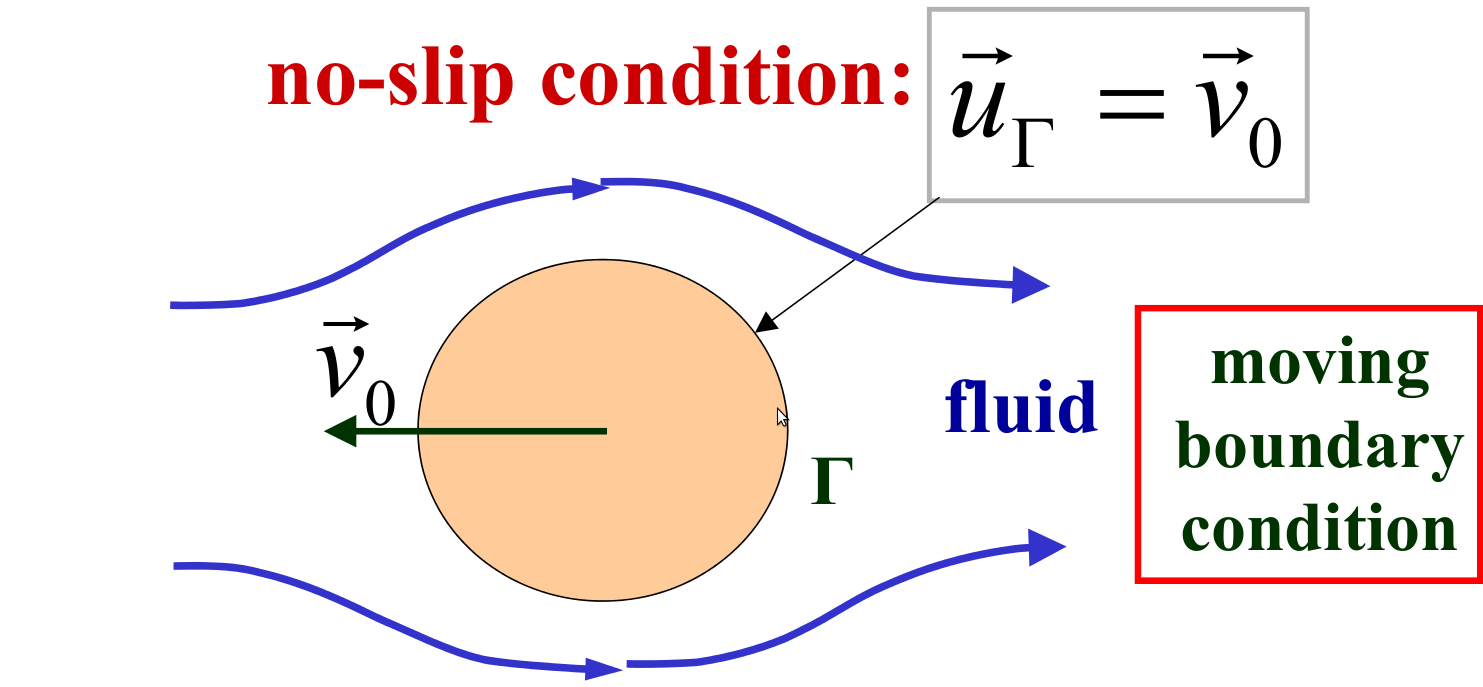
\includegraphics[width=.85\textwidth]{pics/fluid1.png}
    \captionof{figure}{The motion of a particle in a fluid can be determined by computing the interaction of the fluid with the particle's surface.}
    \label{fig:fluid1}
  \end{minipage}
\hfill
  \begin{minipage}{0.05\textwidth}
\,
  \end{minipage}
\end{minipage}
\vspace{0.2cm}

The motion of the fluid (i.e., the Navier-Stokes equations) has to be solved by taking the boundary conditions of the fluid into account. Since the particles that we are considering are moving, the boundaries of the fluid (the particles' surface) are also moving. For each time step the fluid's motion has to be computed, and from the motion of the fluid one obtains the forces to input into the  equations of motion of the particles (e.g. Newton's equations). The total drag force can be obtained by integrating the stress tensor of the fluid over the particles' surface:

\begin{equation}
\vec{F}_D = \int \mat{\Theta} \text{d} \vec{A}
\end{equation}
with he stress tensor of the fluid
\begin{equation}
\mat{\Theta}_{i,j} \equiv - p \delta_{i,j} + \eta\kl{\pder{u_i}{x_j} + \pder{u_j}{x_i}},
\end{equation}
where $\eta$ is the static viscosity. The tensor can be divided into the static and the dynamic part. The static part is dependent on the pressure (scalar) field and the dynamic one is dependent on the velocity (vector) field. If we consider incompressible flows, or at least a pressure that is constant over the particles' surface, $\nabla p$ in \eqref{eq:nseq} disappears and the forces are only dependent on the gradient of the velocity field of the fluid. This is often the case for velocities that are below the speed of sound of the fluid (the velocity at which longitudinal pressure waves propagate). In particular, the forces can be approximated as being proportional to the part of the velocity gradient that is perpendicular  to the surface elements. Discretezing the space around the particle and solving the fluid's velocity gradient is one key to the solution of this problem. It is clear that there are no analitical solutions if not in very special cases. Within some limits (see \cite{drag_law}) The drag law can be approximated as
\begin{equation}
F_D = \frac{\pi\eta^2}{8\rho} C_D Re^2.
\end{equation}
The drag coefficient $C_D$ depends on the velocity of the particle in the fluid and on the density and the viscosity of the fluid. In the so called Stokes limit (for $Re << 1$), the force can be approximated as
\begin{equation}
F_D = 6\pi \eta R u.
\end{equation}
Here $\eta$ is the viscosity of the fluid, $R$ the radius of the particle, $u$ the  velocity of the fluid relative to the particle. For $Re >> 1$ we obtain the Newton's law
\begin{equation}
F_D = 0.22 \pi \rho R^2 u^2.
\end{equation}

These laws are obtained with some simplifications, and this can lead to some substantial deviations in experiments, e.g. due to the particles' shape. Another important factor is the pressure gradient, which we ignored here. This leads to important effects such as lift forces (important in aerodynamics) or the Magnus effect for fast rotating particles. Already In the (analitically) very simple Stokes limit, the computation of multiple particles can become cumbersome: the velocity field of the fluid also depends on the particles' position and velocity. This hydrodynamic problem is similar to a long ranging interaction problem and therefore difficult to solve for many particles \citep{hydropaper}.






\subsection{Discrete Methods}





\subsubsection*{Smoothed Particle Hydrodynamics}


A commonly used technique is \emph{Smoothed Particle Hydrodynamics} (SPH). In this method \citep{sph1,sph2}, the fluid is regarded as a superposition of smoothened particles or localized density fields. These particles are described by \emph{kernel functions} $W$. Their properties are smeared over the smoothing length $h$ by these kernels such that a quantity A is given by:
\begin{equation}
A\kl{r} 
= \int_\Omega{W\kl{\abs{r-r'},h} A\kl{r'} \text{d}r'}
\approx \sum_j{\frac{m_j}{\rho_j} W\kl{\abs{r-r_j},h} A_j}
\end{equation}
The continuum fluid is hence replaced by locally smoothed quantities at discreete coordinates. For this method, space does not have to be discretized and it is therefore suitable for arbitrary shapes of the fluid's boundaries. This is one of the reasons why it first came up in astrophysics, to model the dynamics of galaxies.

\begin{minipage}{.9\textwidth}
  \begin{minipage}{\textwidth}
    \centering
    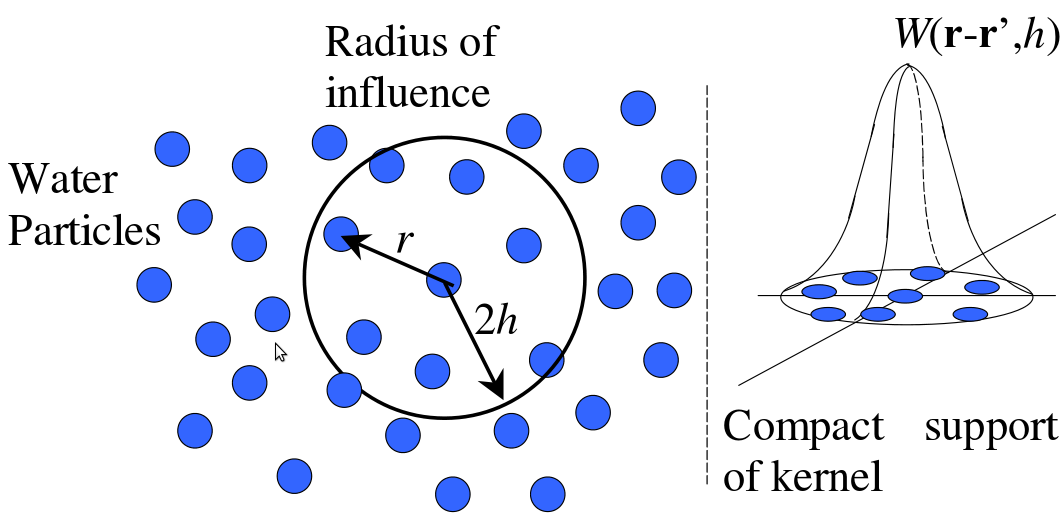
\includegraphics[width=.8\textwidth]{pics/sph1.png}
    \captionof{figure}{The fluid is reduced to a superposition of local kernels.}
    \label{fig:sph1}
  \end{minipage}
\hfill
  \begin{minipage}{0.1\textwidth}
\,
  \end{minipage}
\end{minipage}
\vspace{0.2cm}

Examples for the Kernels could be gaussian distribution or quadratic kernels
\begin{equation*}
W\kl{r,h} = \frac{3}{2\pi h^2}\kl{\frac{1}{4} q^2 -q +1}
\end{equation*}
with $q=\frac{r}{h}$, and $r=\abs{r_a-r_b}$.

There are multiple advantages of doing this: first of all, the gradients can be copmuted analytically. Furthermore, the kernels can be changed without modifying the implementation, thus changing the characteristics of the model with not much coding efford. The results that can be obtained with this technique can be very impressive \citep{sph3}.



\subsubsection*{Dissipative Particle Dynamics}

In a complete different approach, in \emph{Dissipative Particle Dynamics} (DPD), the fluid is simulated as an ensemble of molecules. Since it is impossible to simulate all the molecules, the system is coarse-grained into larger interacting clusters. In a real system on a molecular scale we have momentum conservation but on a macroscopic scale, energy is dissipated (think of the pressure drop when pumping water through a tube). In this case the dissipation can be input artificially \citep{dpd1}. The clustered particles' interaction is modeled with three forces:
\begin{equation}
\vec{F}_i=\sum_{i\neq j}{\kl{\vec{f}_{ij}^{\,C} + \vec{f}_{ij}^{\,R} + \vec{f}_{ij}^{\,D}}},
\end{equation}
where $\vec{f}_{ij}^{\,C}$ represents the conservative forces (e.g., momentum transfer), $\vec{f}_{ij}^{\,R}$ a random force and $\vec{f}_{ij}^{\,D}$ the dissipative forces, proportional to the velocity of the particles. The random forces and the dissipative forces  must be weighted such that the equilibrium distribution is fulfilled at thermal equilibrium \citep{dpd2}.

The main advantage of this technique is the high simplicity of the implementation. The problem is that the viscosity has to be measured, since there are no imput parameter from which this can be calculated. Furthermore, if one inputs artificially some forces, the physics of the system is not respected anymore. The model is therefore not recommended for system in which the equation of state or the correct recovery of energy transport are required. 

\subsubsection*{Stochastic Rotation Dynamics}

In Stochastic Rotation Dynamics (SRD) or Multiparticle Collision Dynamics (MPC), the fluid is represented by particles. Once the space is discretized with a grid, one considers the number of particles in the cells as an site density.  At each time step a pair of particles in the cells is chosen randomly and regarded as a colliding pair, even if they are not on collision course. To simulate the collision, one simply randomly rotates the two particles. The momentum is trivially conserved and macroscopically the system should recover the real physics.



\subsubsection*{Direct Simulation Monte Carlo}

Direct Simulation Monte Carlo (DSMC) \citep{dsmc1,dsmc2} is very popular in aerospace engineering. The reason for this is because the method is very well suited for fluids in which the mean free path of the particles is larger then relevant physical length. In the higher atmosphere the gas is very rarefied, and we have very large Knudsen number due to the diluted fluid.


After the collisions, groups of particles are grouped together and new velocities and temperature are distributed following the equilibrium distribution. This is why this method is called Monte Carlo, even if no real MC computations are involved. For further information, see \citet{dsmc3,dsmc4}.


\newpage

As we saw in this section, very often computations of real systems rely on exotic techniques which microscopically are far from reality (Monte Carlo, lattice gas automata, stochastic rotation and others, like \citet{ballsballs}). The concept of these techniques is that on a macroscopic level, the physical reality is recovered and that they are less expensive than a real molecular dyamics simulation, with realistic potentials. Since everyone of these techniques is based on different assumptions, before using them it is very important to know when and under which conditions these methods converge towards realistic results. Besides this, there is a very wide range of important applications: biology (flow of blood cells, obstructions of arteries, flow through porous membranes, ...), industry (paints, oil stocking,...), geology (sedimentation, erosion, aeolian saltation, ...), aerospace engineering, planet formation, relativistic jet flows...
Although we will not treat the topic further, \emph{computational fluid dynamics} is a very important field of study in which a lot of effort is put today.  The solution of the dynamics of and in various fluids (interstellar dust, liquids, air, atmospheric turbulences, wind turbines...) are fundamental for understanding and studying physical processes and for several applications in engineering. Entire lecture series focus on different aspects of CFD and are recommended for those interested in the topic.











